\section{dayMOPS: Orbits}
\label{orbits}

Orbits are used in a variety of places within dayMOPS (and nightMOPS). We fit orbits (6 parameter Keplerian orbits) to the sets of diasources which make up a track in order to determine which tracks correspond to real moving solar system objects, as the orbit fits provide much tighter constraints on the linkages than the track fits.  After determining an orbit for a movingObject, we identify potential additional detections from both previous observations and future observations by predicting the positions of the movingObject from the orbit, adding those detections to the fit, and re-evaluating the orbit, through the processes of precovery and attribution. We also use orbits and their uncertainties to determine the positions and their uncertainties of known movingObject for nightMOPS. 

Thus, under the general heading of `orbit software' we actually have a variety of needs. These include:
\begin{itemize}
{\item Ephemeris generation. This is software to generate positions, velocities, and magnitudes of moving objects at a particular time from a given orbital element distribution.  This is needed for nightMOPS and for precovery and attribution. }
{\item Orbit propagation. This is software to propagate orbital elements backwards and forwards in time; the resulting changes in the orbital elements can be minor (updating the mean anomaly, for example) but over a longer timespan can be major (changing semi-major axis and eccentricity due to the influence of other planets, for example). This is often bundled with ephemeris generation, but is not necessarily quite the same. This is needed for ephemeris generation, but may also be important for detecting duplicate movingObjects (a single movingObject discovered at two separate times during the survey). }
{\item Initial Orbit Determination. This is software to fit a preliminary orbit to a set of detections, usually only used when there are only a few detections such as when we first discover a movingObject. This is needed for the orbit determination stage of dayMOPS. }
{\item Differential Orbit Determination.  This is software to fit a full orbit to a set of detections, usually incorporating all available observations and leveraging the initial orbit determination fit into a fit that includes error bars. Sometimes IOD and DOD are packaged together in orbit determination software, but mathematically these are usually separate processes with different assumptions on the underlying orbit. For example, IOD may assume that the detections represent an object near perihelion, while DOD may relax that assumption and try to fit for the perihelion location and mean anomaly. }
\end{itemize}

Often all of these capabilities are bound together in a single distributed software package, but this is not necessarily the case. Furthermore, it may be to LSST's advantage to use different packages for different needs, if there are speed differences. For example, ephemeris generation and orbit propagation may be tasks that translate well to GPU architecture, given the repetitious and math intensive nature of the calculations, while IOD and DOD may not due to the individualized nature of each fit. 

\subsection{Orbit packages}

At present, the number of available open-source software packages is limited. OpenOrb, by Mikael Granvik, provides Fortran95 code with limited python interfaces. OrbFit, by Andrea Milani, provides Fortran95 code only. Both of these software packages provide all the functionality above, although with varying disadvantages. There may be other open-source packages available, but these are the main two we have investigated, and seem to be the only two that provide all functionality required for all types of solar system objects. 

One of the main differences between OpenOrb and OrbFit is their approach to IOD, and in particular, DOD. OpenOrb uses statistical ranging while OrbFit is based on geometric orbit fits for DOD.  A extremely simplified description of statistical ranging would be: generate many possible orbits for a particular set of detections and see which one fits the observations the best. This has the advantage that it will (to the limits of the parameter space which is explored) find the best fit orbit, including being able to distinguish between NEOs and MBAs with short observational arcs. It will return a probability distribution function of all likely orbits, even if they are not connected in orbital parameter space. This makes it scientifically most accurate in calculating an orbit, and gives the best estimate of whether an object is truly an NEO or not. It has the disadvantage that it is calculating ephemerides for many possible orbits and comparing those predictions to the observed detections, to see which one 'fits the observations best'. This makes it compute-intensive, and as a result, slow.
An extremely simplified description of geometric orbit fits would be: take the observed detections and fit an ellipse through those detections, using an analytic formula. This has the advantage that it is extremely fast in comparison to statistical ranging and could identify orbits well enough to recover the objects at a later time, even if the orbit determination was incorrect. It has the disadvantage that a single orbit, with (most likely) incorrect errors (because generally the error space is non-gaussian) is returned, and in particular, NEO orbits may be assigned to MBA objects at particular solar elongations.  There is likely also differences in IOD, although these details are less clear (to me). 

OpenOrb's code exceeds 60,000 lines in the main portion of the software, and provides two different python libraries for interacting with this code. One is an f2py library which handles ephemeris generation (with and without errors) and orbit propgation, while another is a custom python interface (which may be out of date, depending on if API changes have occured) for IOD and DOD.  OrbFit's codebase exceeds 160,000 lines, so is also not a simple program (there are multiple ways to find best options for the orbit fit, particularly for short arcs, beyond the simple ellipse). Note that the version of OrbFit being used by PS is not quite the same as the open-source version: Milani rewrote some of the code to be faster. There are no python bindings, and OrbFit interacts with data through text files (separate files for each object). 

A rough comparison of the relative speed of orbit determination using each of these methods gives:
\begin{itemize}
{\item OpenOrb 20s / track (estimates from JM) [10s for ranging (IOD) with a subset of detections, 10s LSL (DOD) with all linked detections] }
{\item OrbFit 0.005s / track (estimates from PS)}
\end{itemize}
Obviously, this difference in orbit fitting is significant. It is likely that the requirements for OpenOrb could be tuned with better understanding of the ranging and least-squares stages, but it seems unlikely that it will be as fast as OrbFit (or even within a few orders of magnitude).  Beyond considerations of the speed of orbit fitting, there are also considerations of ease of use and integration with the LSST stack. This is where OrbFit is difficult, as requiring text files for each object will not scale well for the number of objects expected in LSST or for our computing platform. In addition, it would be difficult for LSST to maintain these codes independently of the original authors. 

Orbit determination is performed per-track and is thus trivially parallelizable. In addition, unlike the linking phases, these algorithms require little memory overhead. 

In terms of ephemeris generation, both packages appear similar. We have done some tests to determine the timing requirements for ephemeris generation with OpenOrb and find 
\begin{equation}
\text{Time}_{10,000\text{\,objects}} (s) \approx 0.7(\frac{s}{\text{day}}) (\text{Days\,from\,Orbit\,Epoch}) + 3.5 (s)
\end{equation}
on a macbook pro (see Figure~\ref{scalingEphemeris}). The major things to note here are that the time required to generate an ephemeris increases as the difference between the orbital epoch and the time of the requested ephemeris increases (due to the need to propagate the orbit to the time of the ephemeris), and that there is some overhead due to reading in the JPL binary files that describe the position of the Earth and other major planets and writing out the outputs. In addition, the time required to generate ephemerides for N objects scales as O(N). 


\begin{figure}[h]
\begin{center}
  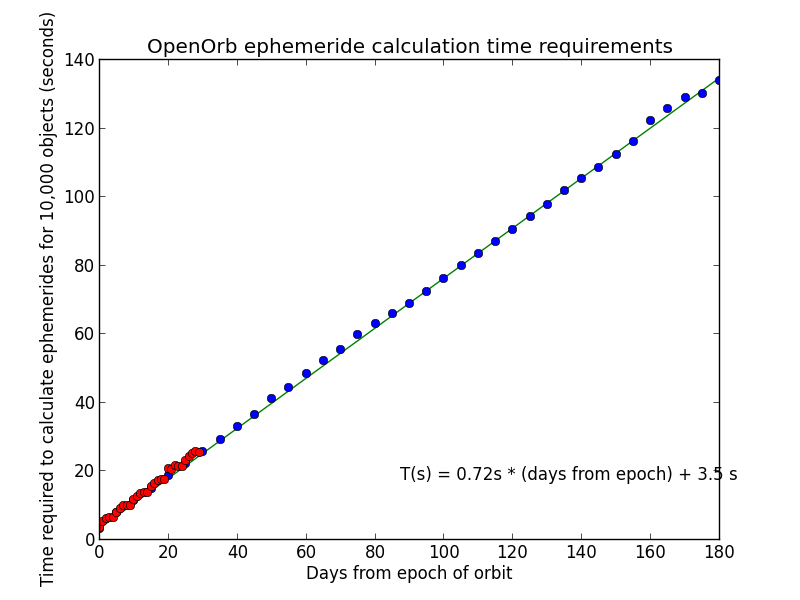
\includegraphics[width=6in]{illustrations/openorb_ephems.png}
\end{center}
\caption[OpenOrb ephemeris computation time requirement.]{Results of a test of the time required to generate ephemerides for 12,078 objects (scaled to 10,000 objects for the plot) using OpenOrb. }
\label{scalingEphemeris}
\end{figure}
